% Organização sugerida para uma introdução de plano de estágio

\chapter{Diagrama de caso de uso}\label{sec:2}

O diagrama de caso de uso é uma das partes fundamentais do projeto, pois é com ele que serão definidos os requisitos funcionais de forma clara do sistema. Na Figura~\ref{fig:caso-de-uso} são apresentados os principais atores e funcionalidades da aplicação.

\begin{figure}[H]
    \caption{Caso de uso}
    \label{fig:caso-de-uso}
    \centering
    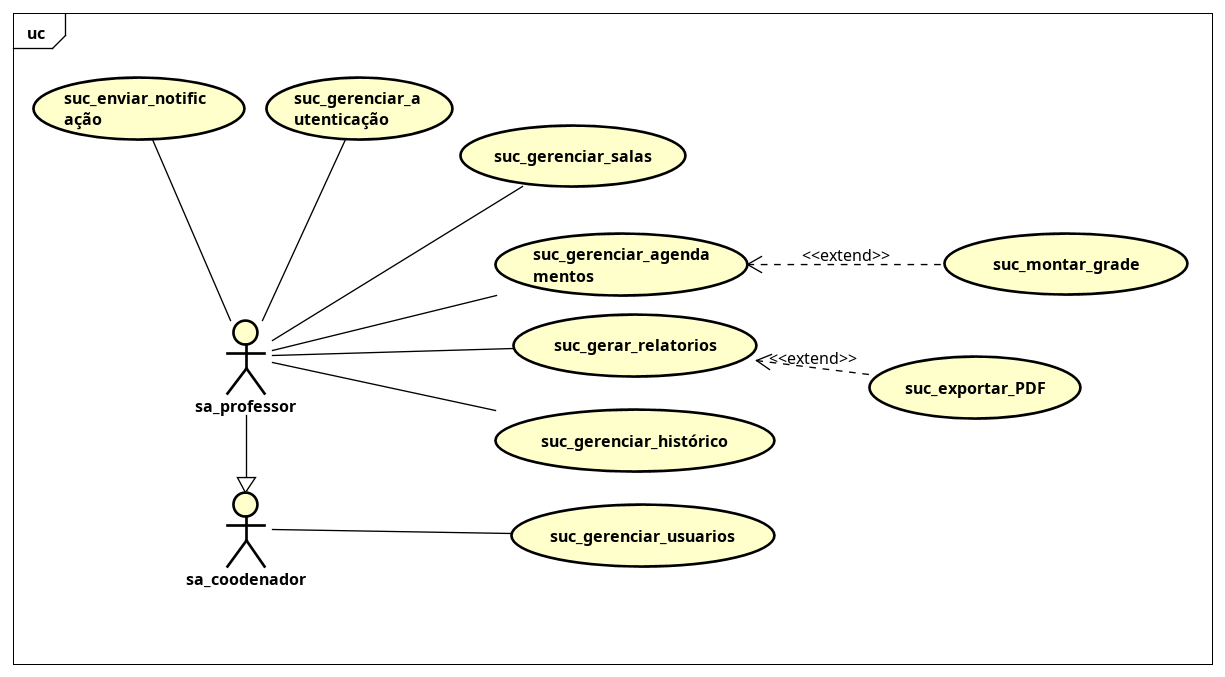
\includegraphics[width=1\textwidth]{imagens/caso_de_uso.png}

    {\footnotesize \textbf{Fonte:} O autor.}
\end{figure}

\section{Casos de uso}

\begin{description}
    \item[\textbf{suc\_enviar\_notificacao}] Permite ao sistema enviar notificações aos usuários sobre atualizações, lembretes e eventos importantes.

    \item[\textbf{suc\_gerenciar\_autenticacao}] Permite realizar login, logout e controle de acesso dos usuários no sistema.

    \item[\textbf{suc\_gerenciar\_salas}] Permite cadastrar, editar, remover e consultar as salas disponíveis.

    \item[\textbf{suc\_gerenciar\_agendamentos}] Permite criar, atualizar, cancelar e visualizar agendamentos de salas.

    \item[\textbf{suc\_gerar\_relatorios}] Permite emitir relatórios com informações consolidadas sobre uso, agendamentos e histórico do sistema.

    \item[\textbf{suc\_gerenciar\_histórico}] Permite consultar e acompanhar o histórico de ações, reservas e alterações realizadas.

    \item[\textbf{suc\_gerenciar\_usuarios}] Permite cadastrar, editar, remover e consultar usuários do sistema.

    \item[\textbf{suc\_exportar\_PDF}] Permite exportar documentos, relatórios ou comprovantes em formato PDF.

    \item[\textbf{suc\_montar\_grade}] Permite organizar e estruturar a grade de horários ou ocupação das salas.
\end{description}

\clearpage
\section{Telas}
As telas foram feitas com objetivo de serem simples e acessíveis para os usuários, além de proverem ferramentas necessárias para o uso avançado do sistema.

\Needspace{0.7\textheight}
\subsection{Tela de login}
Como demonstrado em Figura~\ref{fig:tela-login}, será solicitado do usuário, suas credencias, no caso o seu email e senha para acesso.

\begin{figure}[H]
    \caption{Tela de login}
    \label{fig:tela-login}
    \centering
    \makebox[\textwidth][c]{%
        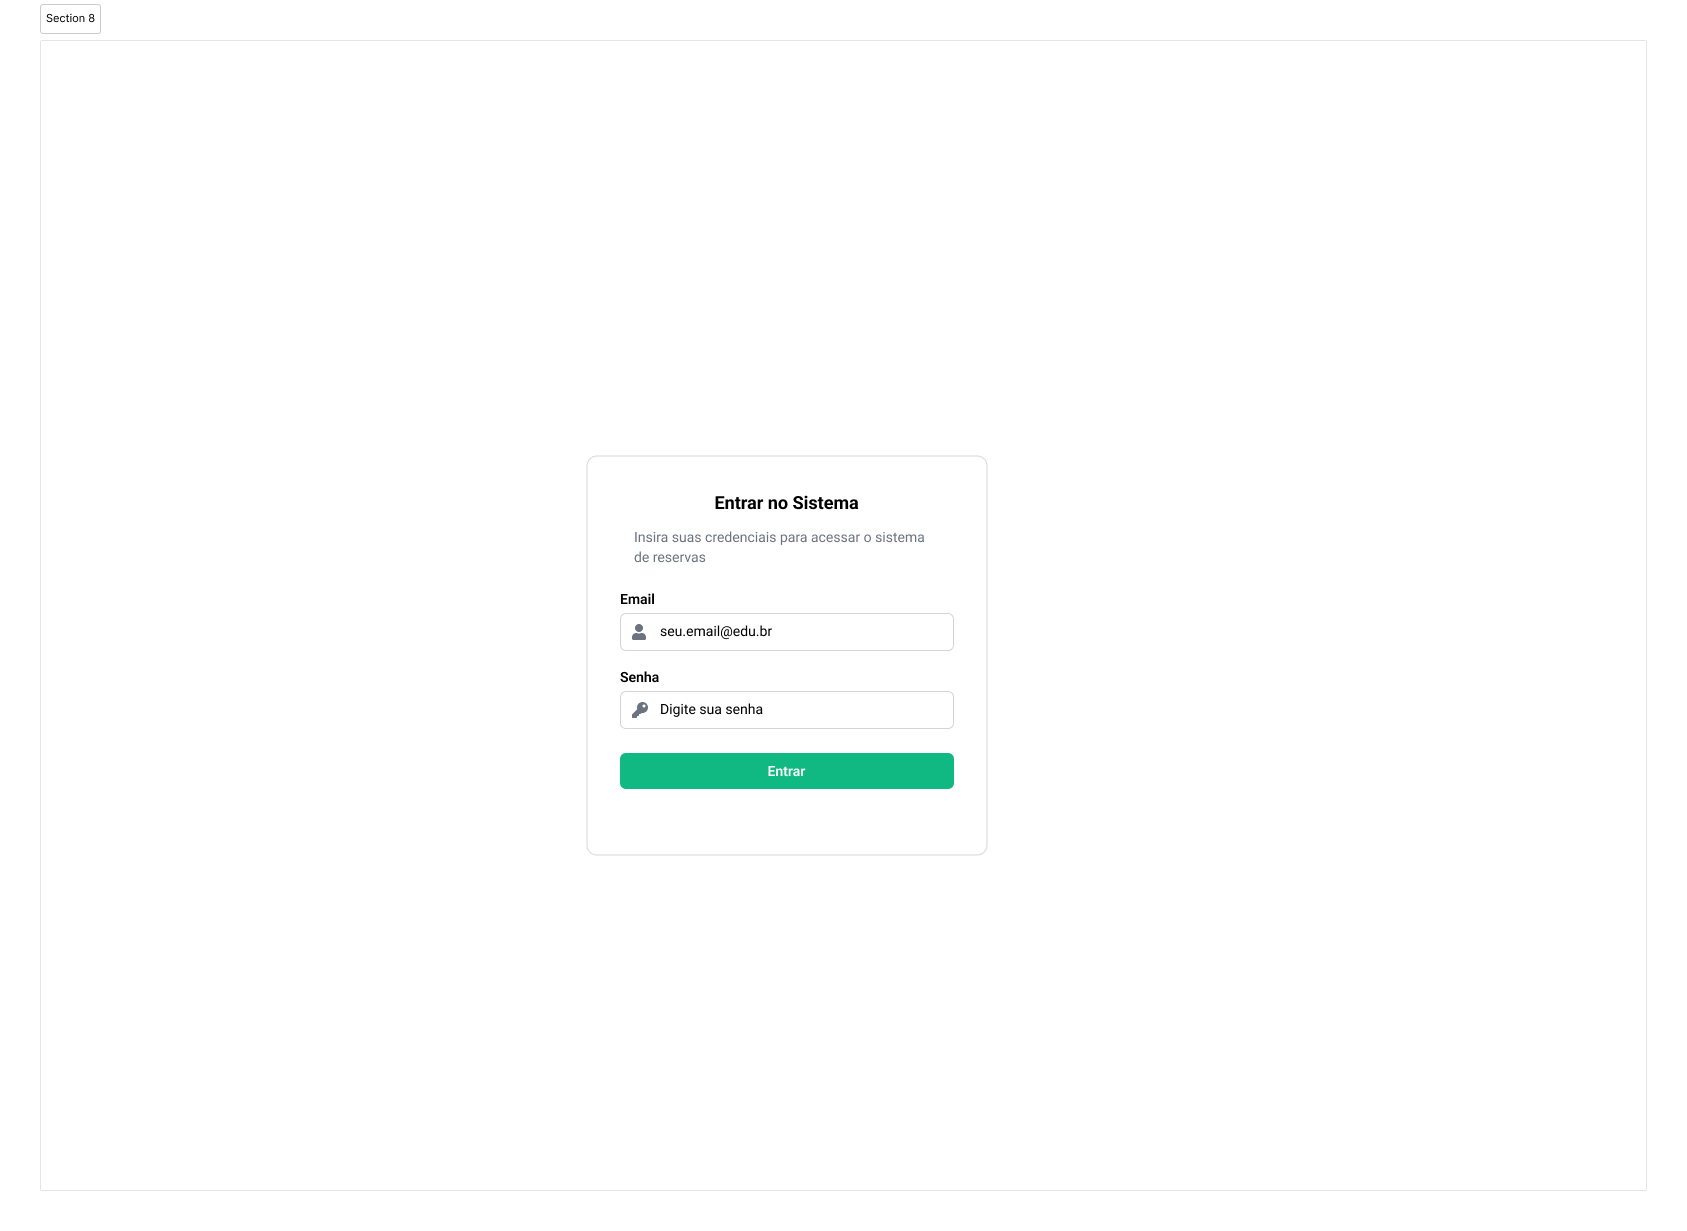
\includegraphics[width=1.5\textwidth,trim=5cm 12cm 6cm 15cm,clip]{imagens/telas/login.png}
    }
    {\footnotesize \textbf{Fonte:} O autor.}
\end{figure}

\Needspace{0.7\textheight}
\subsection{Tela de gerenciar salas}
Em Figura~\ref{fig:tela-gerenciar-salas}, o usuário pode visualizar as salas cadastradas e executar ações de gerenciamento, como adicionar, editar ou remover registros.

\begin{figure}[H]
    \caption{Tela de gerenciar salas}
    \label{fig:tela-gerenciar-salas}
    \centering
    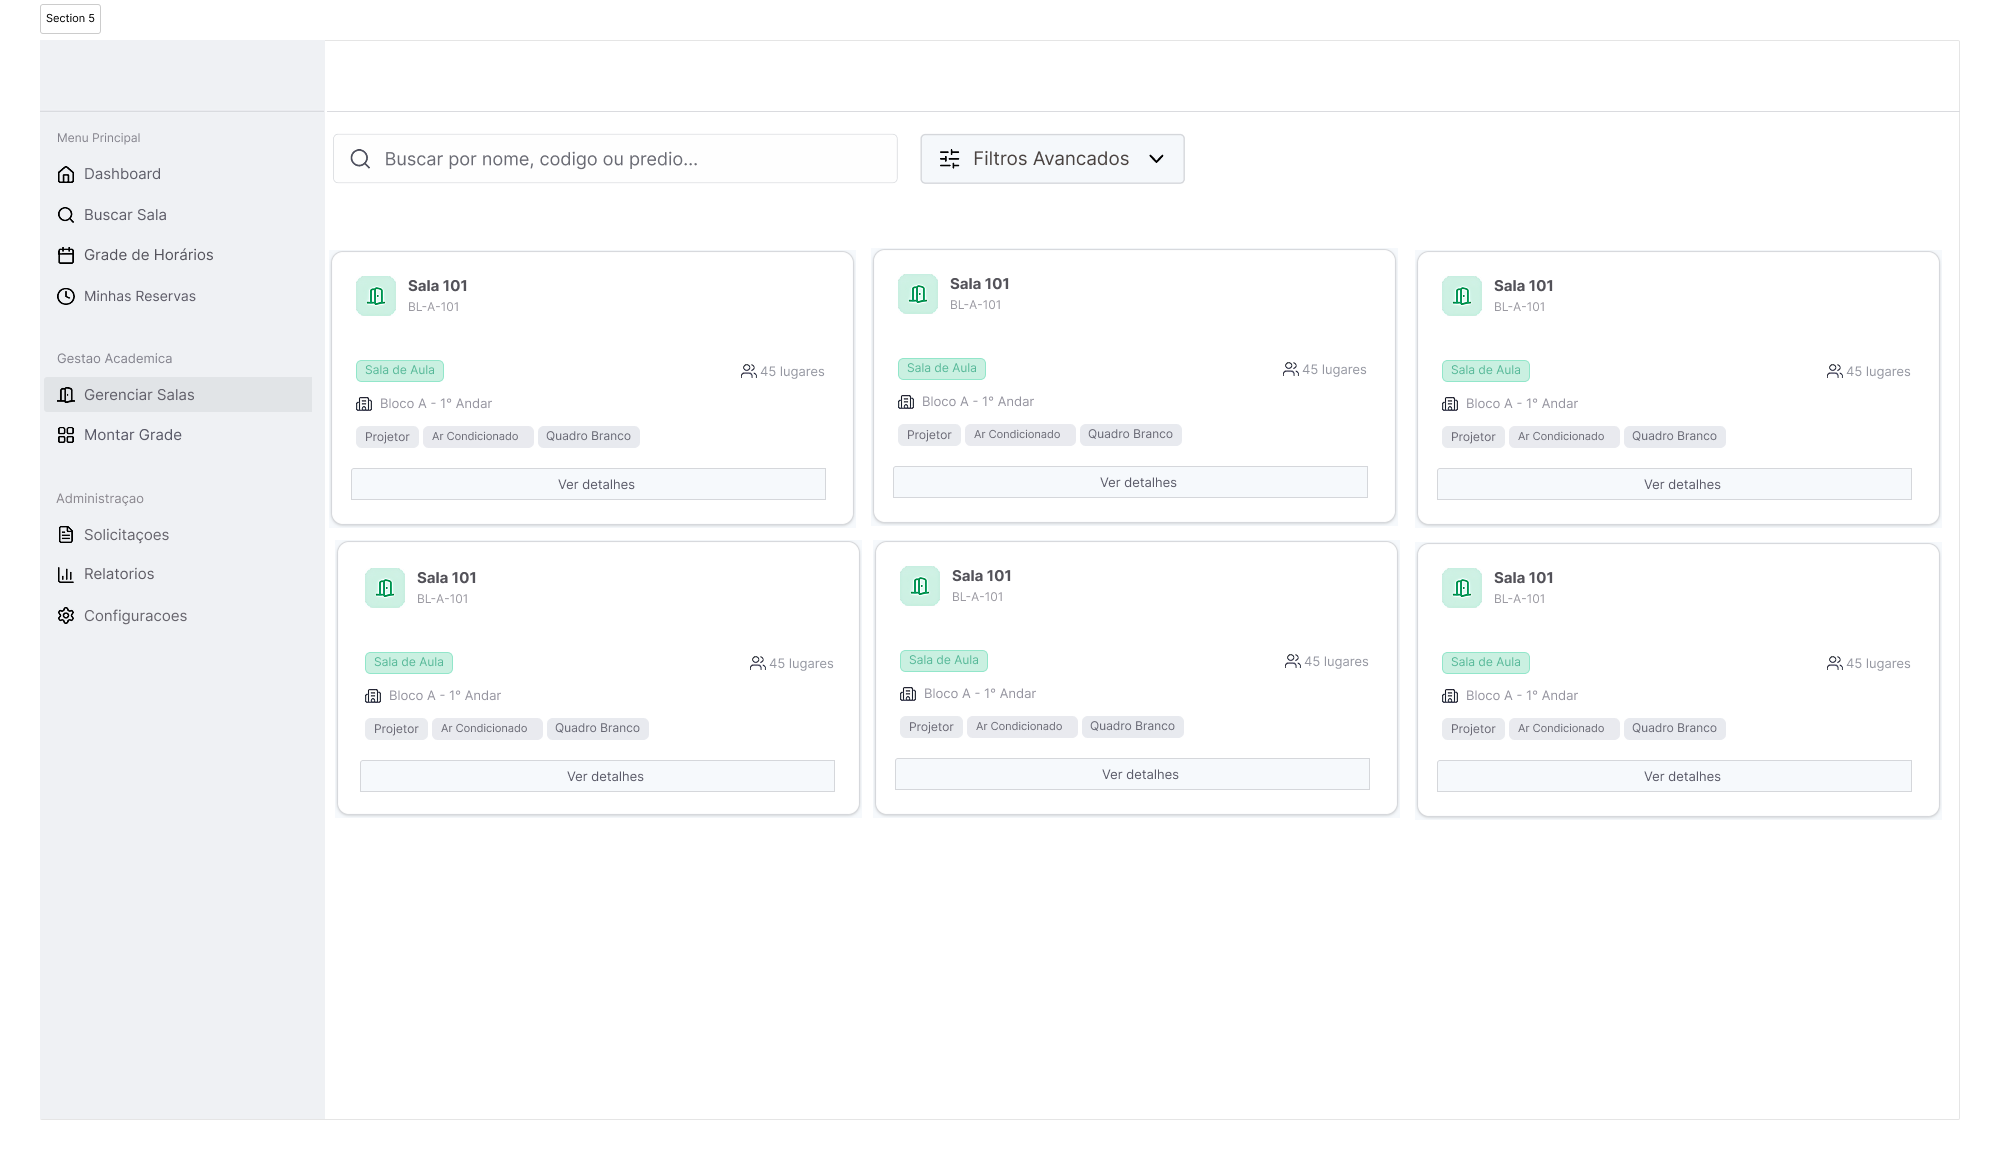
\includegraphics[width=1\textwidth]{imagens/telas/gerenciar-salas.png}
    {\footnotesize \textbf{Fonte:} O autor.}
\end{figure}

\Needspace{0.7\textheight}
\subsection{Tela de buscar sala}
Em Figura~\ref{fig:tela-buscar-sala}, esta tela permite consultar todas as salas, facilitando a localização de ambientes conforme a necessidade do usuário.

\begin{figure}[H]
    \caption{Tela de buscar sala}
    \label{fig:tela-buscar-sala}
    \centering
    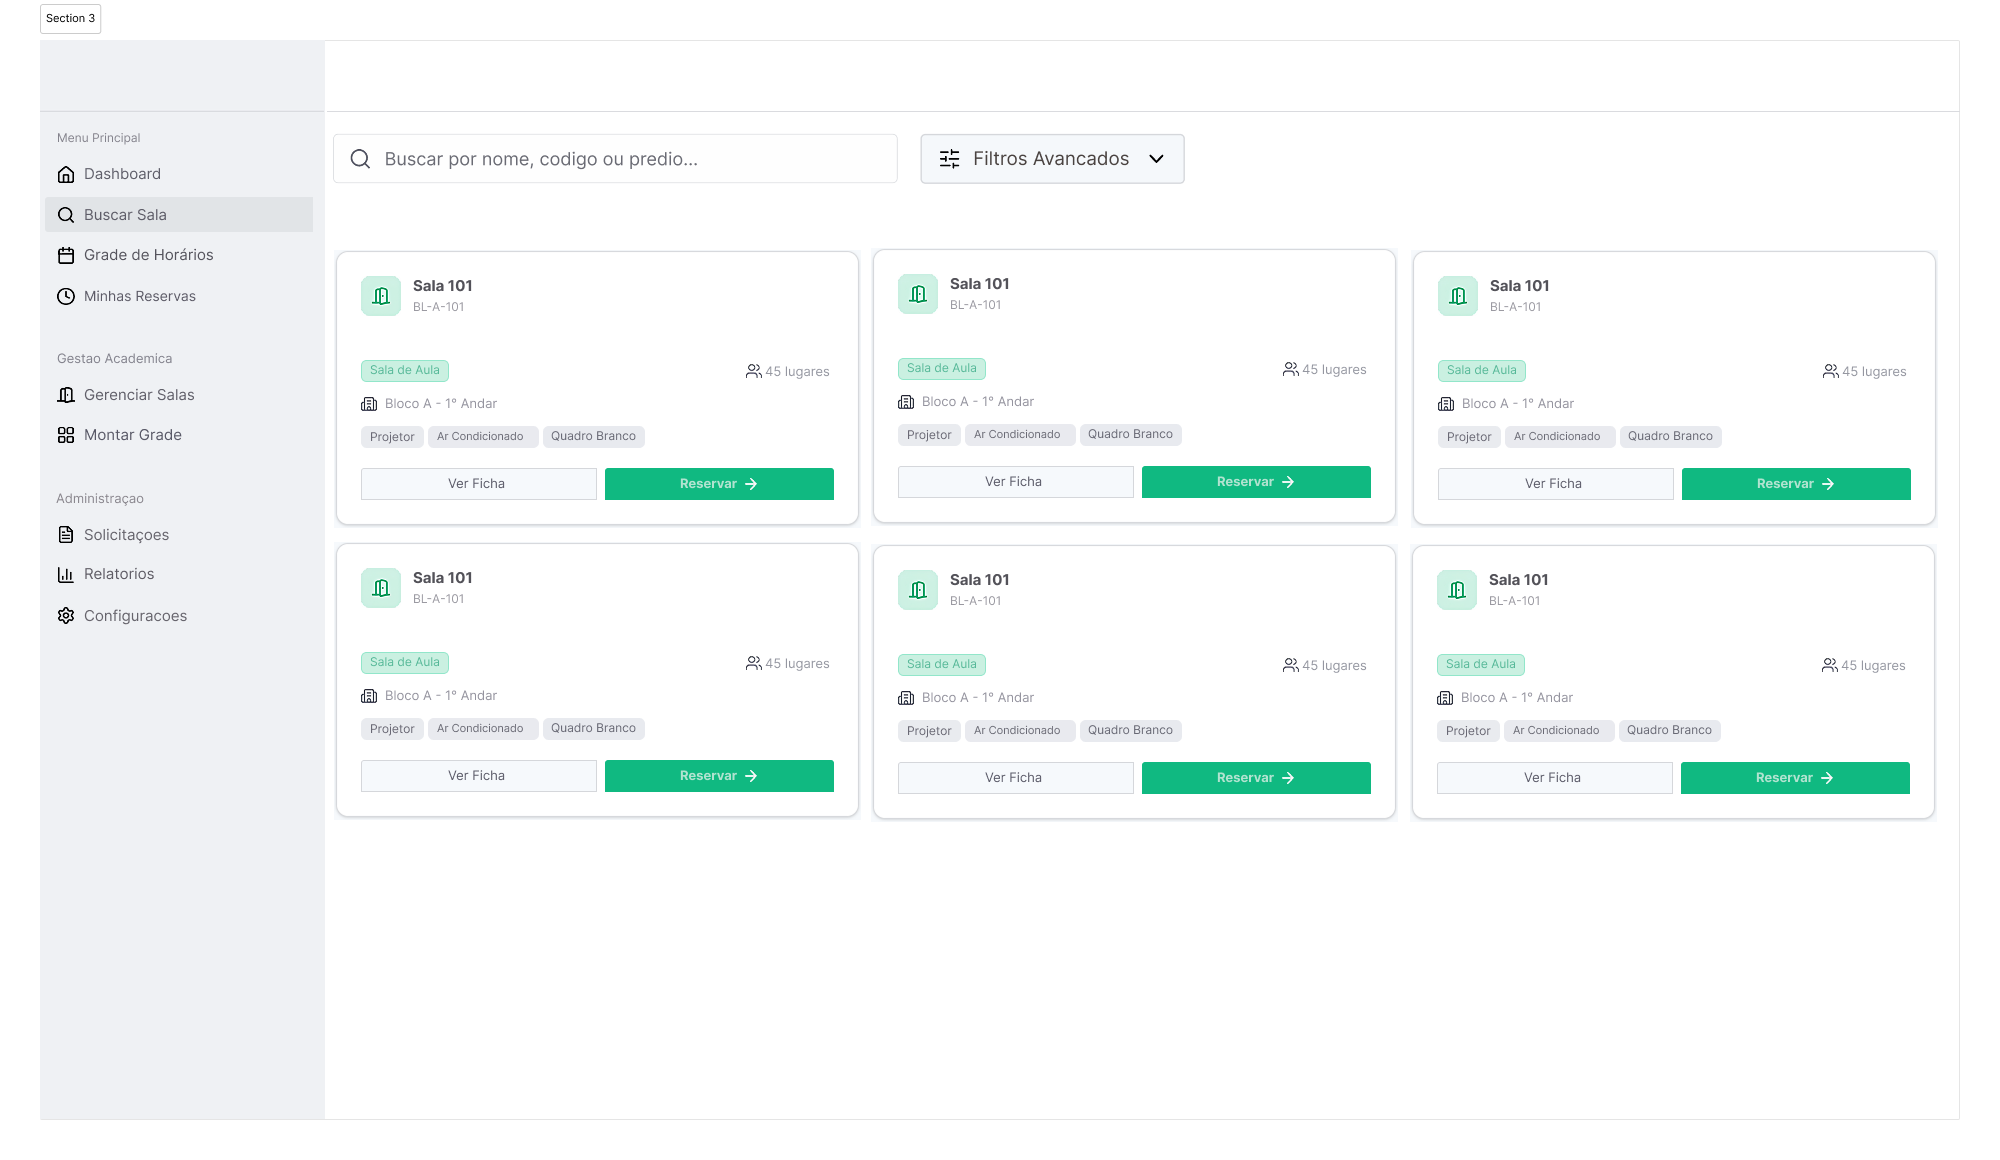
\includegraphics[width=1\textwidth]{imagens/telas/buscar-sala.png}
    {\footnotesize \textbf{Fonte:} O autor.}
\end{figure}

\Needspace{0.7\textheight}
\subsection{Tela de minhas reservas}
Em Figura~\ref{fig:tela-minhas-reservas}, o usuário acompanha as reservas realizadas, podendo consultar informações importantes sobre seus agendamentos.

\begin{figure}[H]
    \caption{Tela de minhas reservas}
    \label{fig:tela-minhas-reservas}
    \centering
    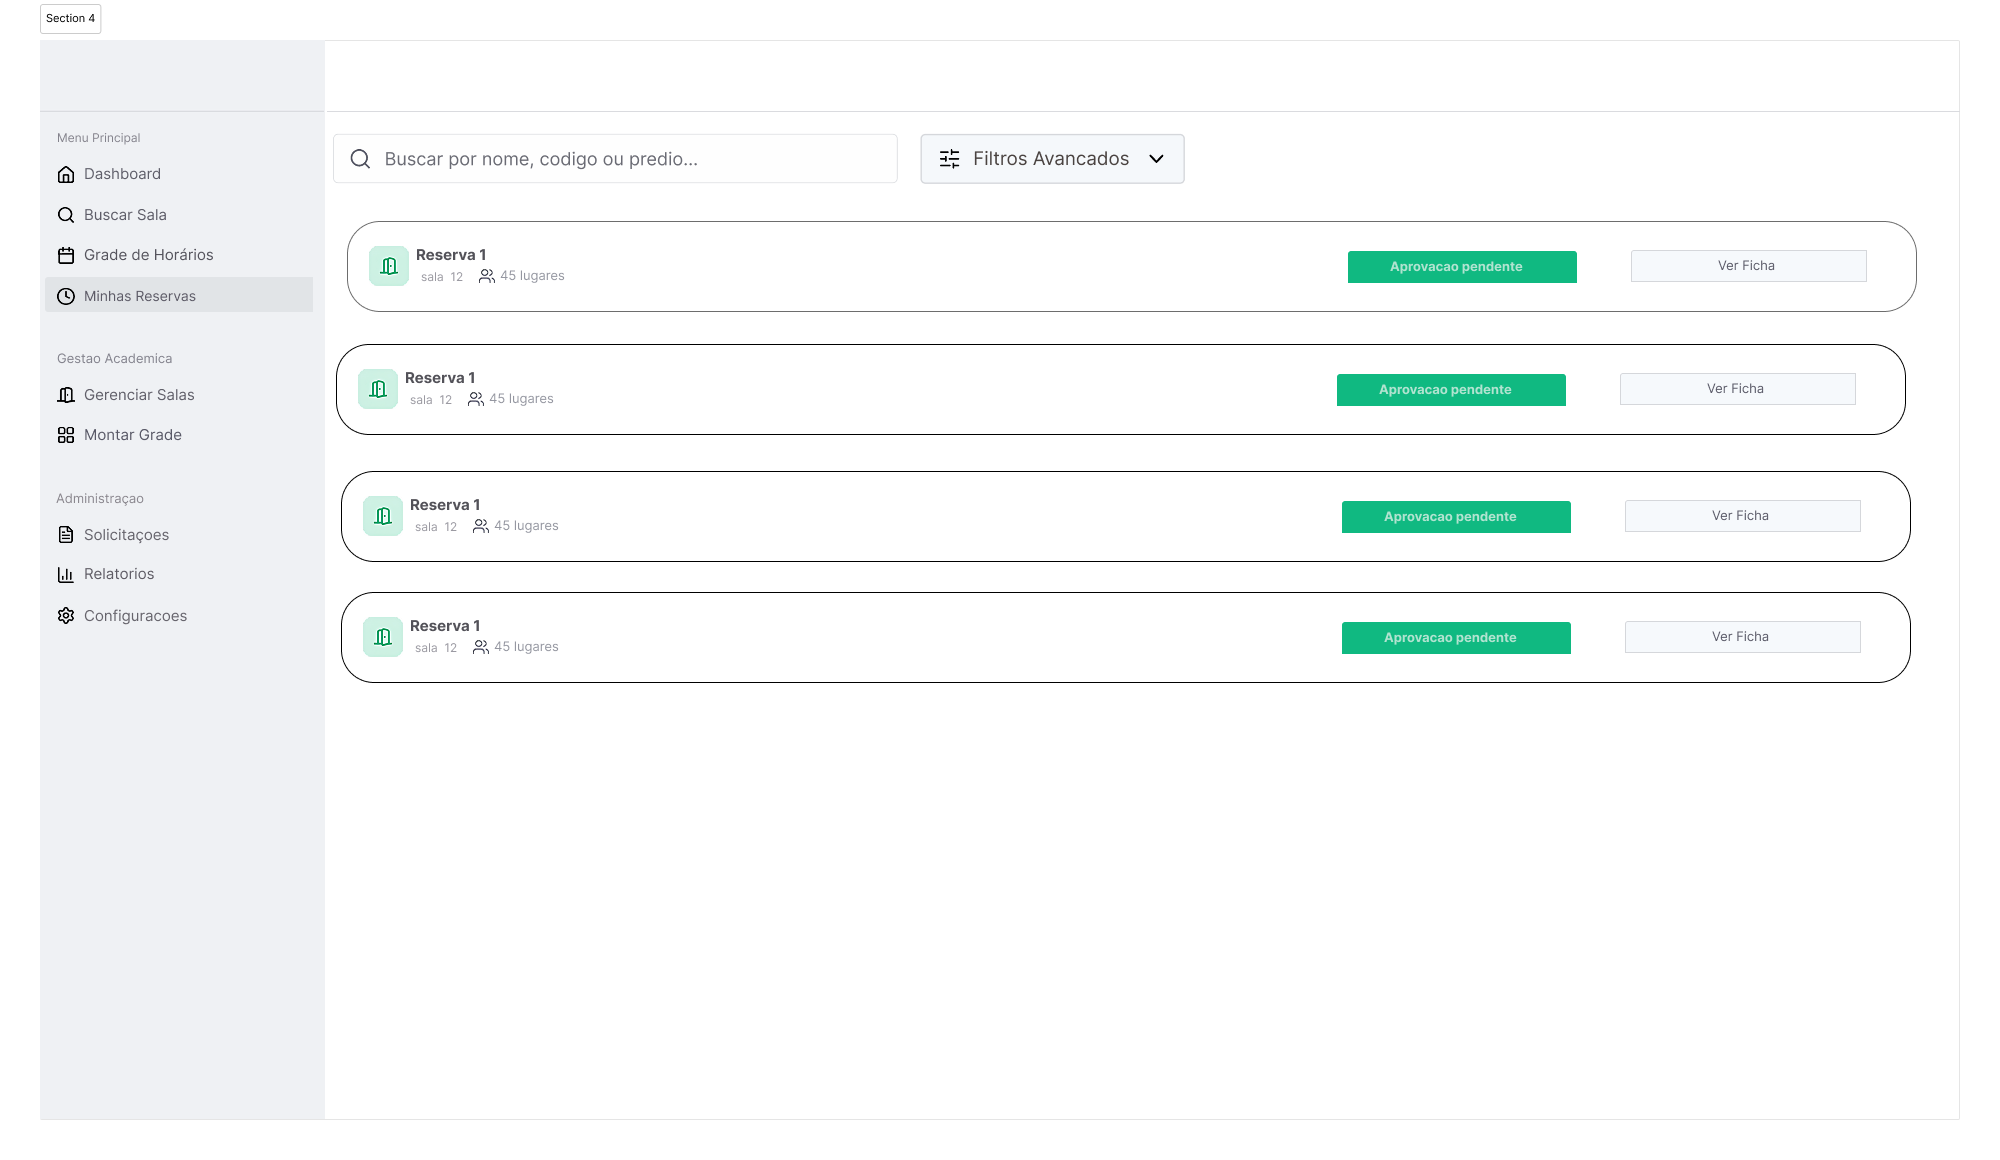
\includegraphics[width=1\textwidth]{imagens/telas/minhas-reservas.png}
    {\footnotesize \textbf{Fonte:} O autor.}
\end{figure}

\Needspace{0.7\textheight}
\subsection{Tela de solicitações}
Em Figura~\ref{fig:tela-solicitacoes}, esta tela apresenta as solicitações relacionadas ao sistema, permitindo ao usuário acompanhar pedidos e seus respectivos status.

\begin{figure}[H]
    \caption{Tela de solicitações}
    \label{fig:tela-solicitacoes}
    \centering
    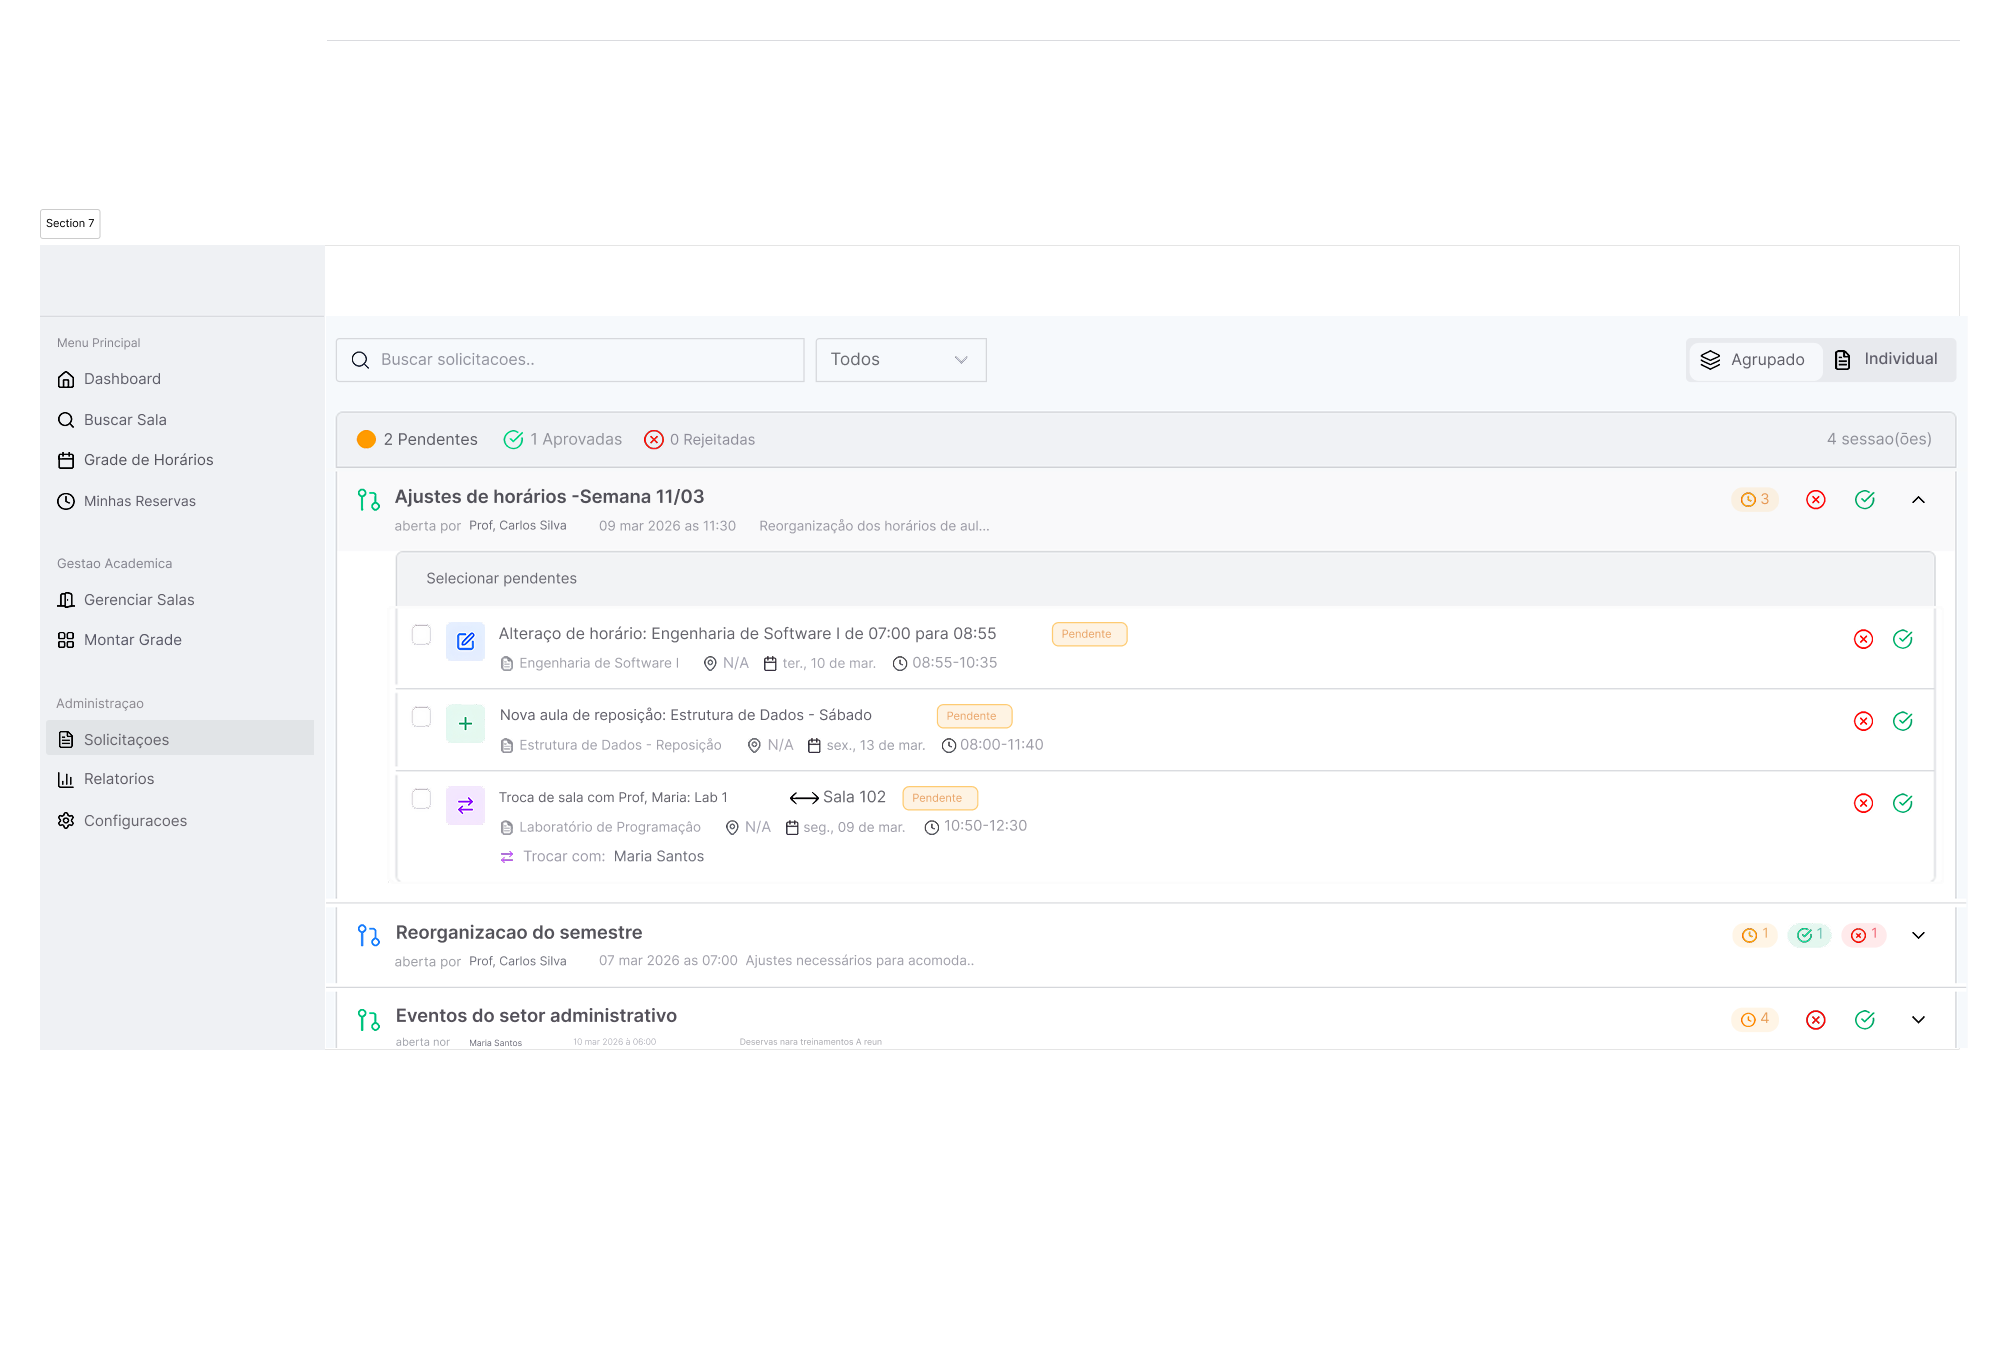
\includegraphics[width=1\textwidth]{imagens/telas/solicitacoes.png}
    {\footnotesize \textbf{Fonte:} O autor.}
\end{figure}

\Needspace{0.7\textheight}
\subsection{Tela de grade de horários}
Em Figura~\ref{fig:tela-grade-horarios}, a tela de grade de horários exibe a organização temporal das salas, ajudando na visualização da ocupação e disponibilidade.

\begin{figure}[H]
    \caption{Tela de grade de horários}
    \label{fig:tela-grade-horarios}
    \centering
    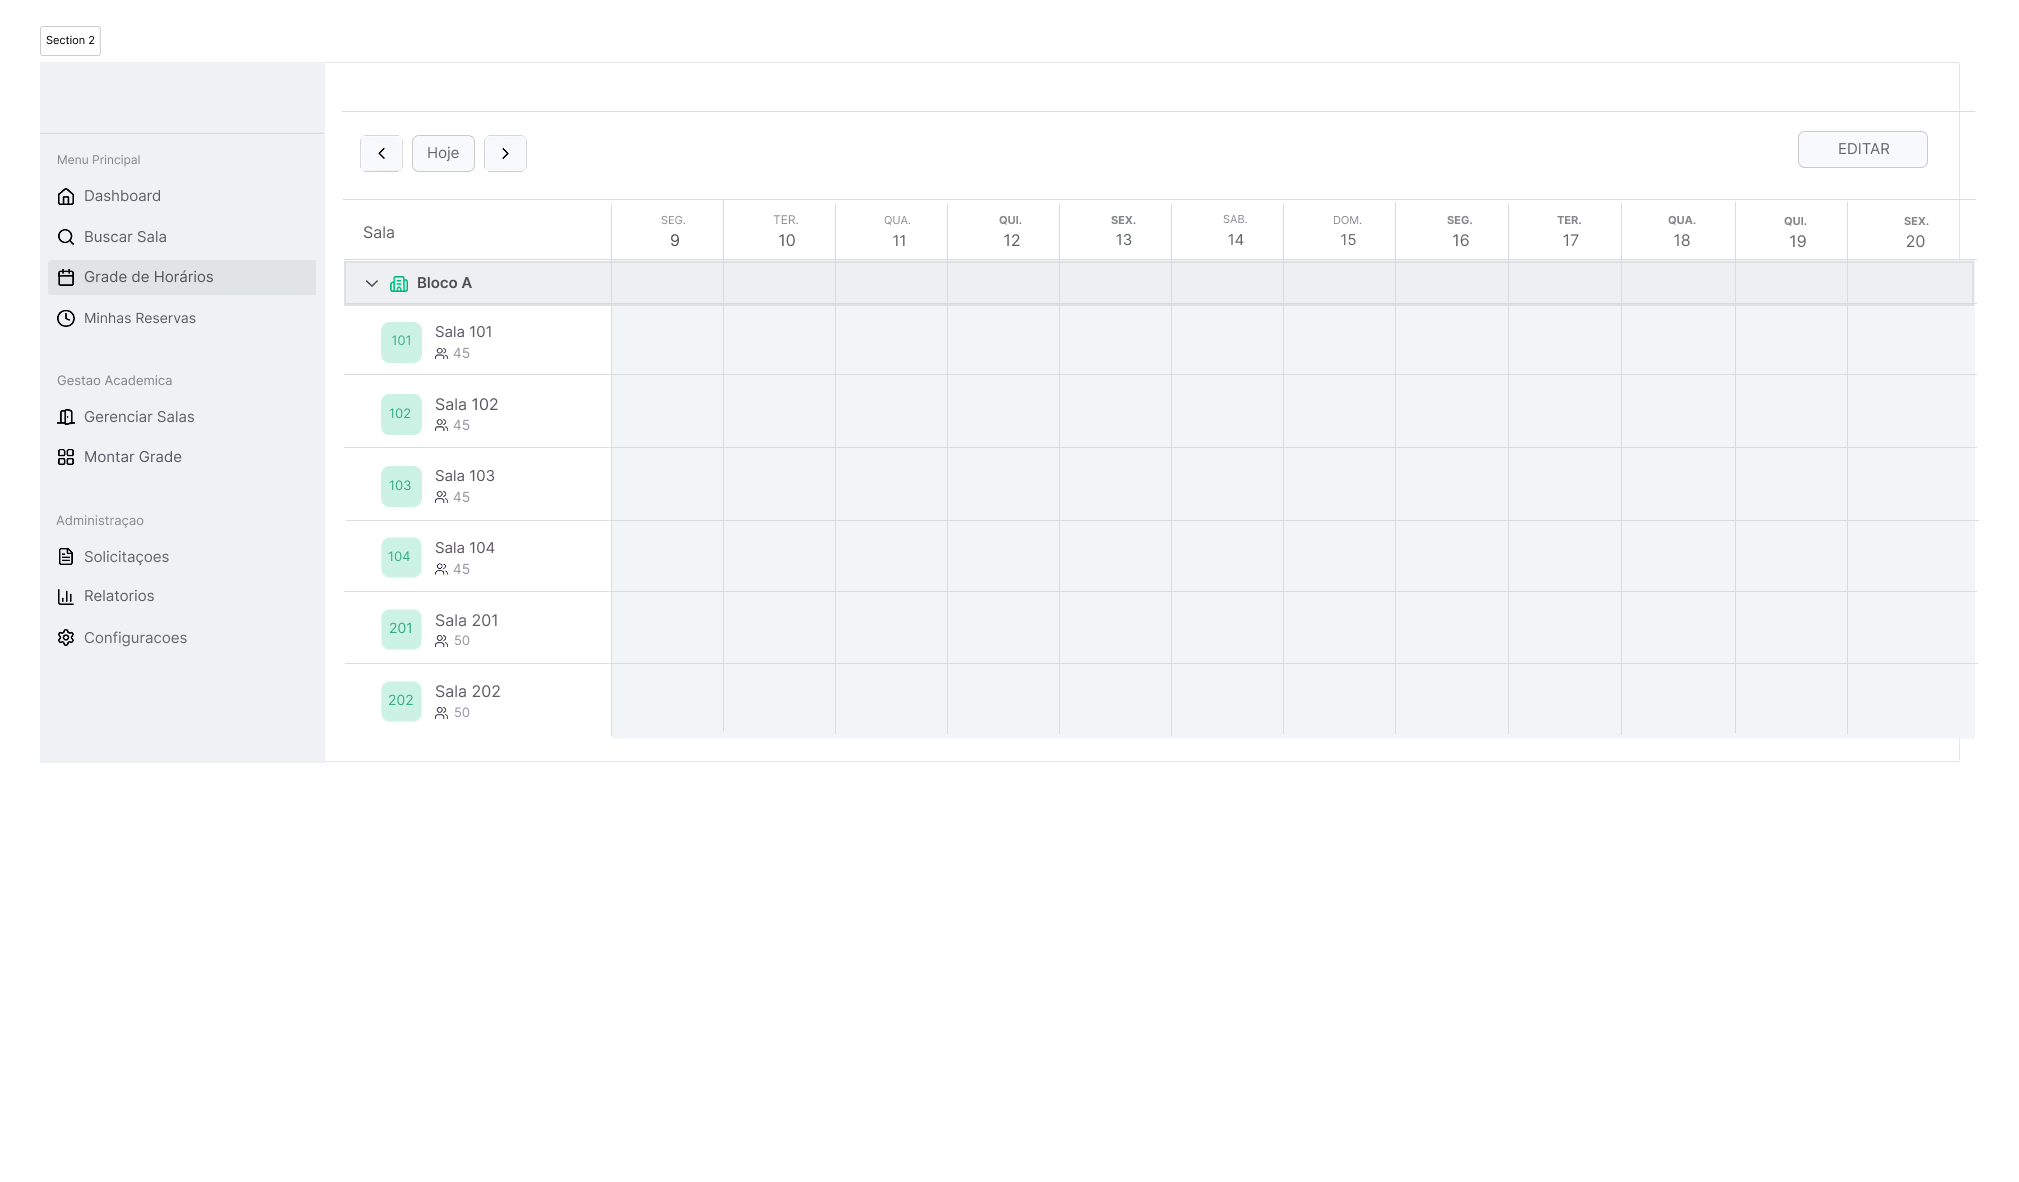
\includegraphics[width=1\textwidth]{imagens/telas/grade-horarios.png}
    {\footnotesize \textbf{Fonte:} O autor.}
\end{figure}

\Needspace{0.7\textheight}
\subsection{Tela de montar grade}
Em Figura~\ref{fig:tela-montar-grade}, o usuário pode estruturar a grade de horários das salas, organizando os períodos de uso conforme as demandas existentes.

\begin{figure}[H]
    \caption{Tela de montar grade}
    \label{fig:tela-montar-grade}
    \centering
    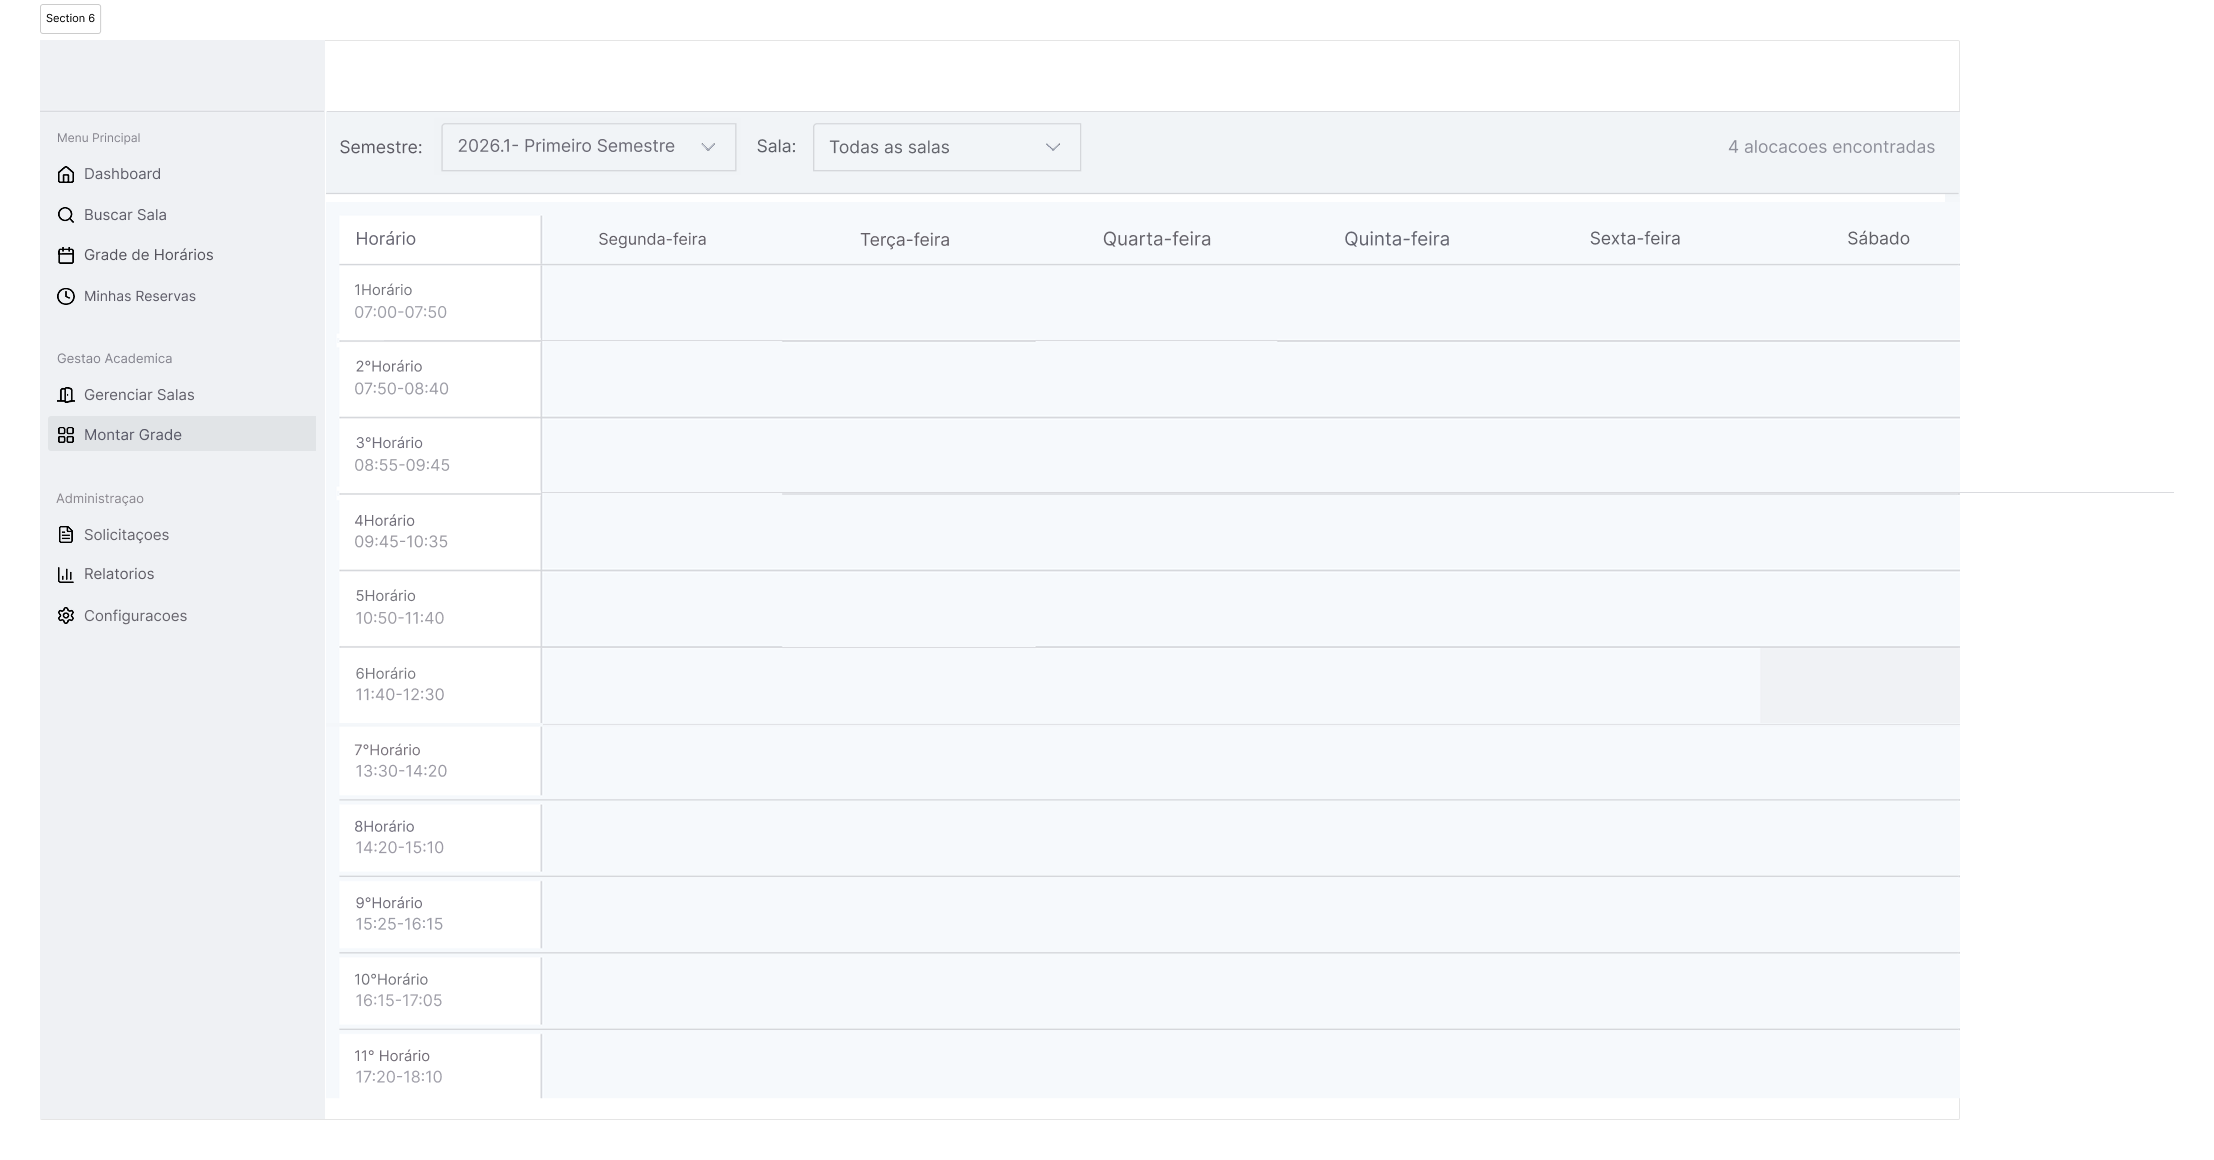
\includegraphics[width=1\textwidth]{imagens/telas/montar-grade.png}
    {\footnotesize \textbf{Fonte:} O autor.}
\end{figure}
